\section{Experiment Design}

\begin{frame}{Development and the Environment}
\begin{columns}
\column{0.5\textwidth}
neglecting environmental influence
\begin{align*}
\vec{p} = f(\vec{g})
\end{align*}
\column{0.5\textwidth}
considering environmental influence
\begin{align*}
\vec{p} = f(\vec{g}, \vec{e})
\end{align*}
\end{columns}
\end{frame}

\begin{frame}{Development and the Environment: Direct Plasticity}
  \begin{figure} \label{fig:elephant_developmental_perturbation}
  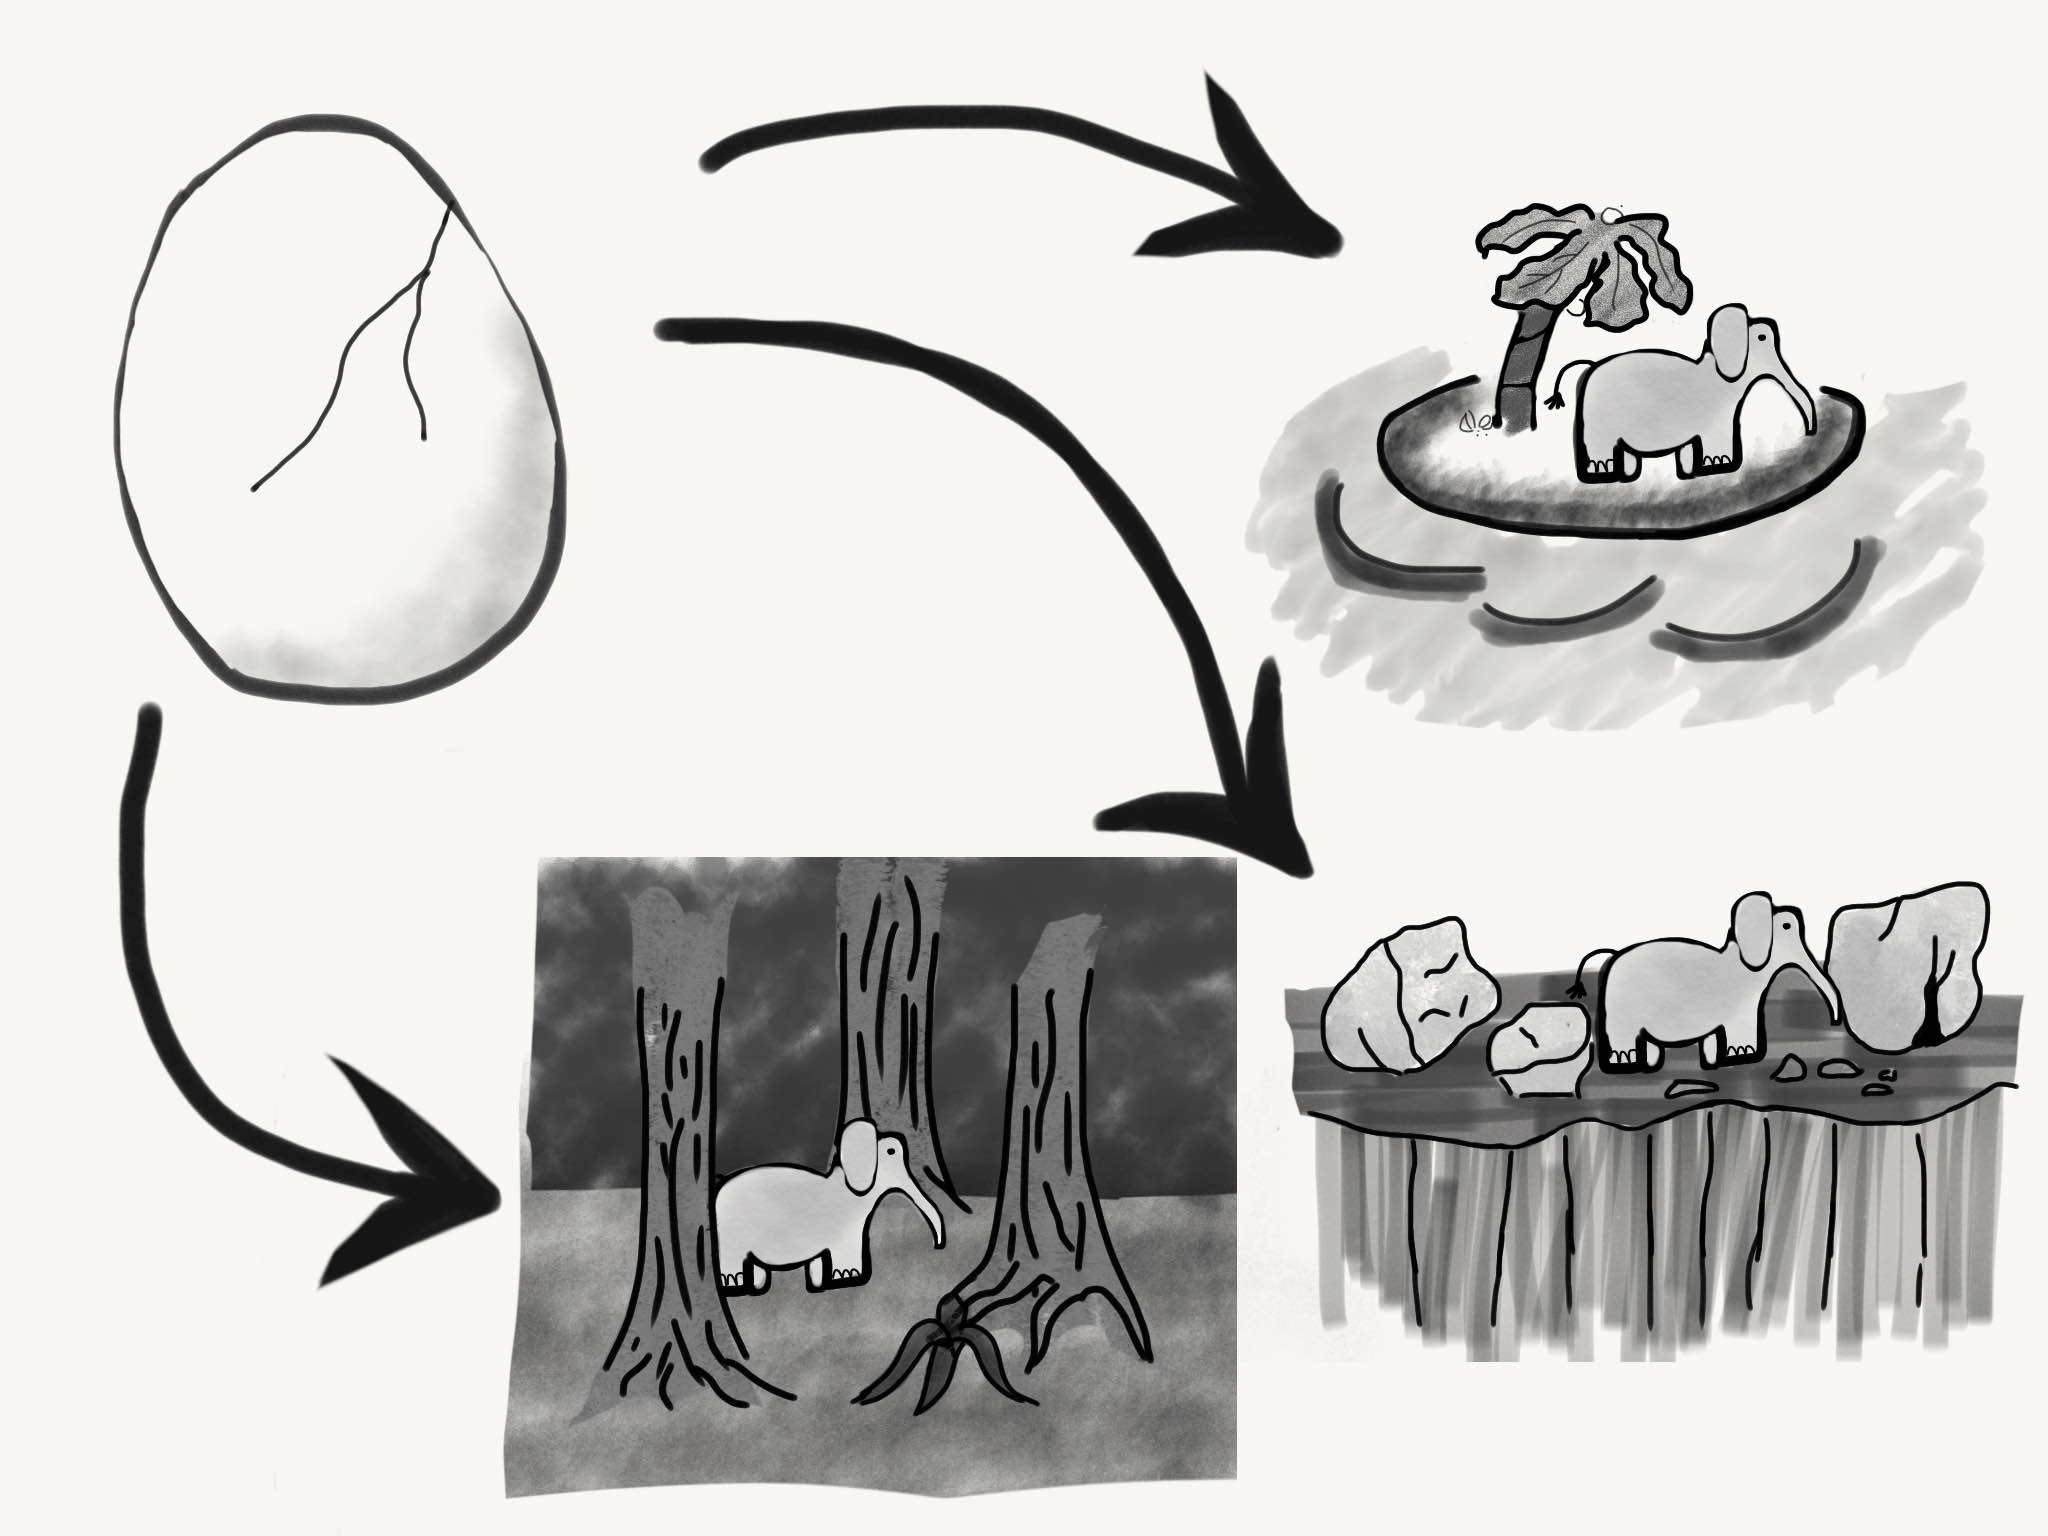
\includegraphics[width=0.8\textwidth]{img/elephant_developmental_perturbation.jpg}
  \captionsetup{singlelinecheck=off,justification=raggedright}

  \caption{An illustration of canalization against environmental perturbation}
\end{figure}
\end{frame}

\begin{frame}{Development and the Environment: Direct Plasticity}
goal is $\dot{\vec{g}}$ such that
\begin{align*}
\vec{p} \approx f(\dot{\vec{g}}, \vec{e})  \approx f(\dot{\vec{g}}, \vec{e} + \bm{\vec{n}})
\end{align*}
\end{frame}

\begin{frame}{Development and the Environment: Indirect Plasticity}
  \begin{figure} \label{figs/plant_developmental_perturbation}
  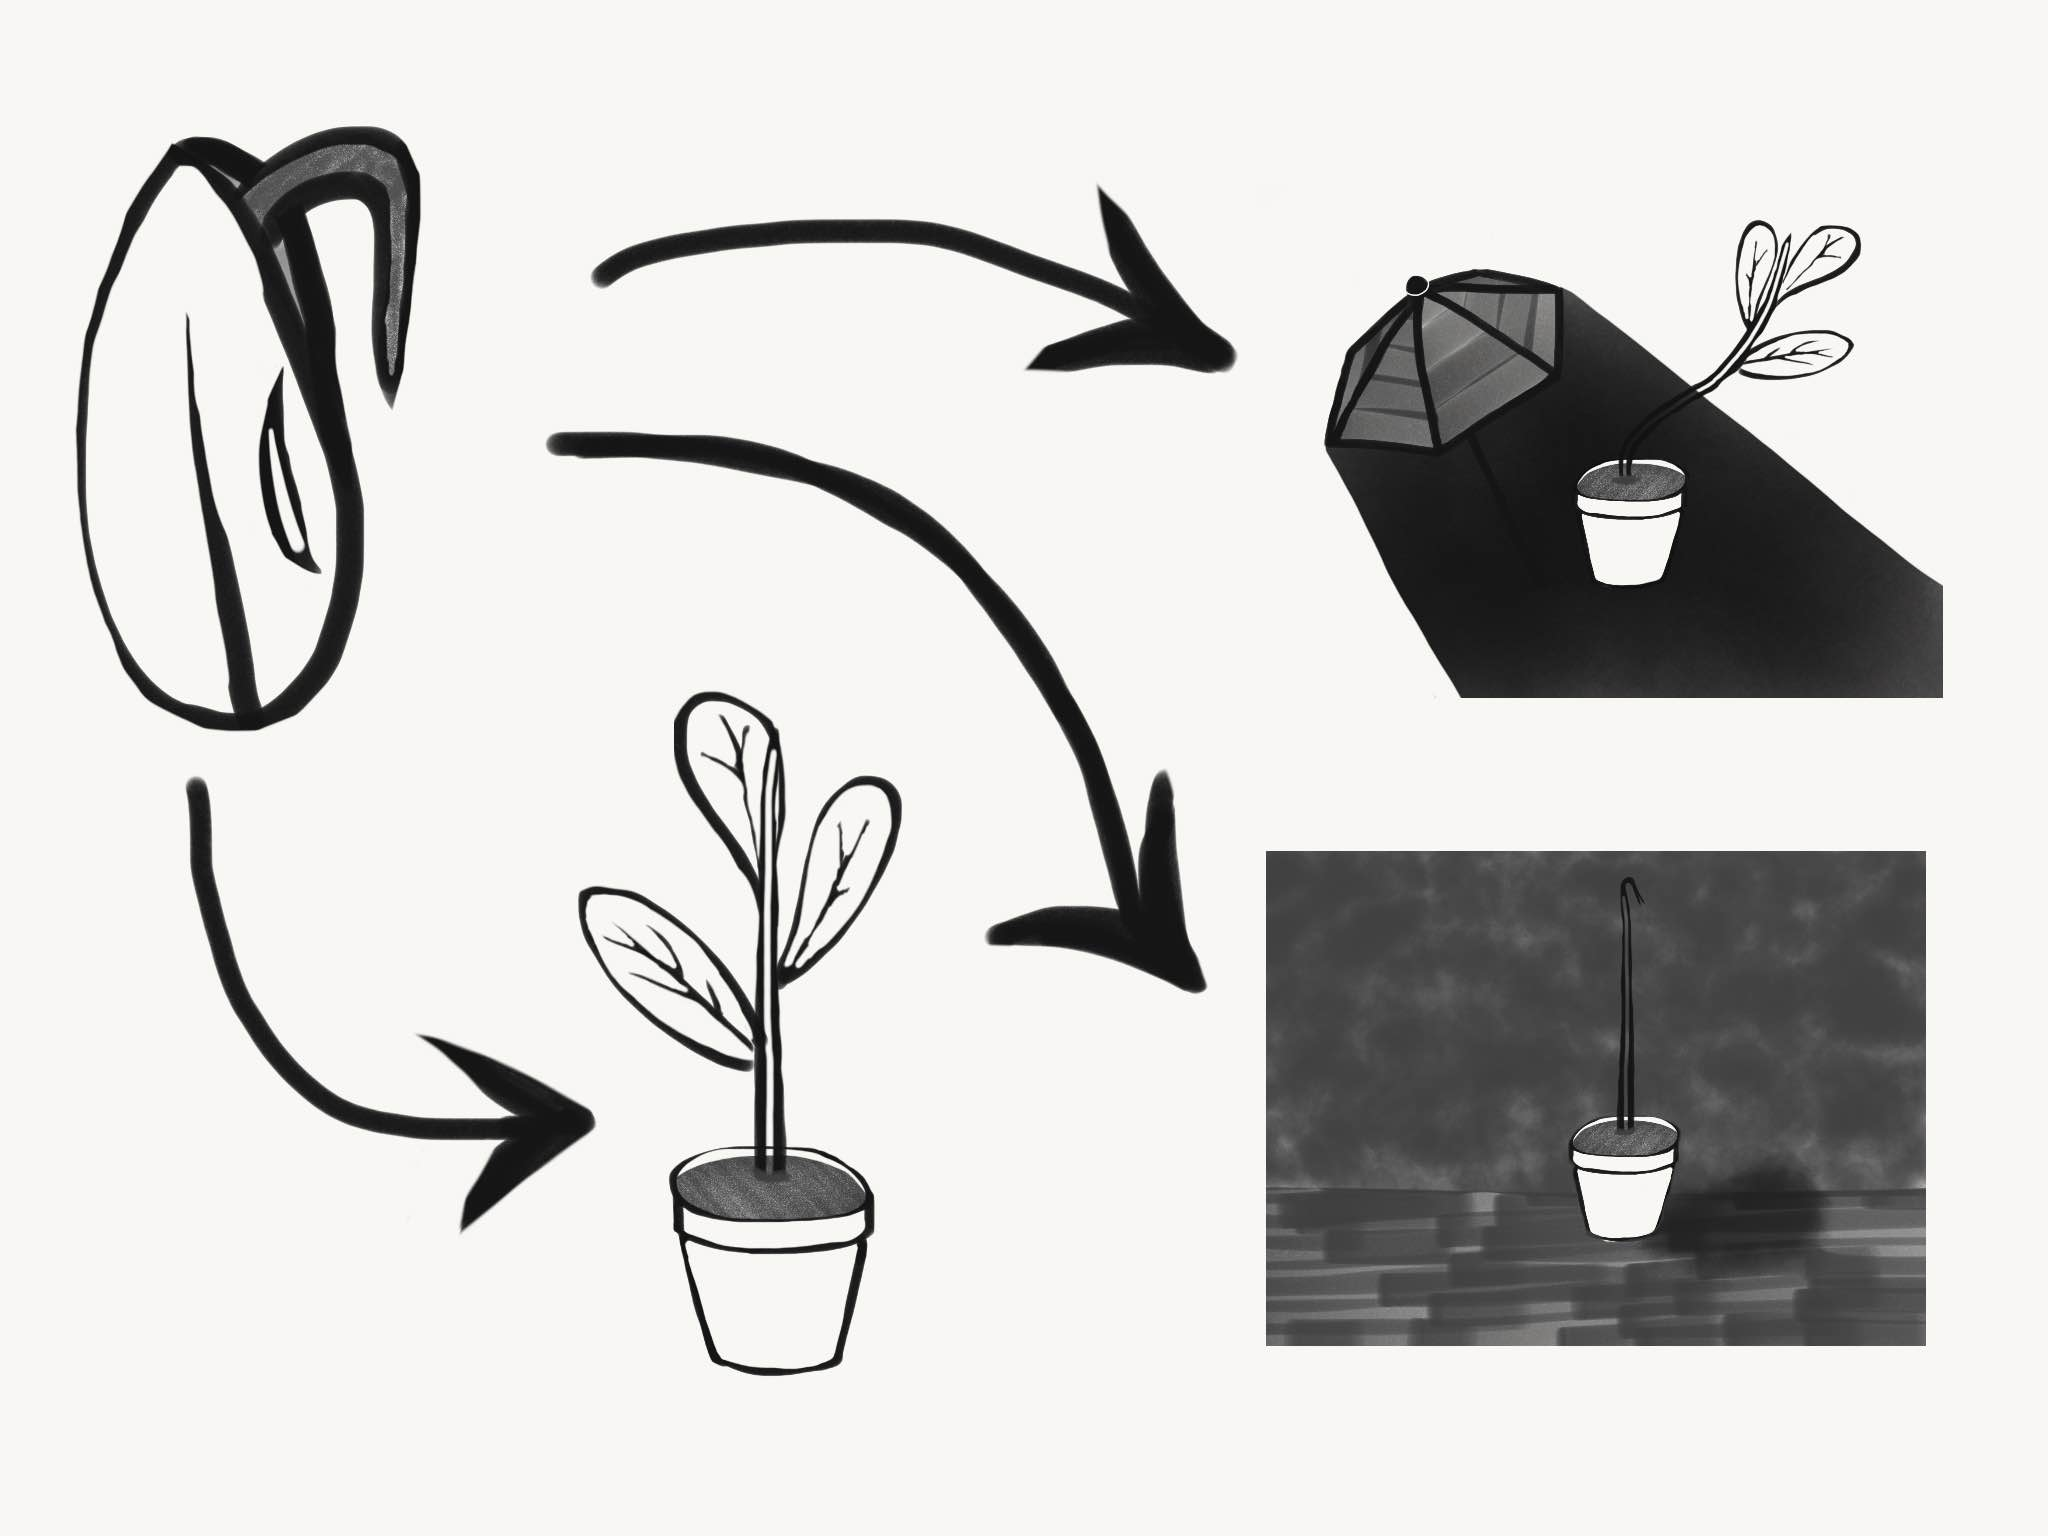
\includegraphics[width=0.8\textwidth]{img/plant_developmental_perturbation.jpg}
  \captionsetup{singlelinecheck=off,justification=raggedright}
  \caption{An illustration alternate phenotypes expressed based on environmental signals}
\end{figure}

\end{frame}

\begin{frame}{Development and the Environment: Indirect Plasticity}
goal is $\dot{\vec{g}}$ such that:
\begin{align*}
\vec{p}_1 &\approx f(\hat{\vec{g}}, \vec{e} + \vec{e}_1) \\
\vec{p}_2 &\approx f(\hat{\vec{g}}, \vec{e} + \vec{e}_2) \\
&\vdotswithin{\approx} \\
\vec{p}_s &\approx f(\hat{\vec{g}}, \vec{e} + \vec{e}_s)
\end{align*}
\end{frame}

\begin{frame}{GRN Models}
  \begin{itemize}
    \item Model A \cite{Wilder2015ReconcilingEvolvability}
	 \begin{align*}
    	W_{i,j} \in \{-1,0,1\} \\
        S_i \in \{0,1\}
    \end{align*}
    \begin{align*}
    S_i(t+1) = 
      \begin{cases}
      1 & \text{if } \sum_{j=1}^{k} W_{ji}S_j(t) > 0 \\
      0 & \text{otherwise.}
      \end{cases}
    \end{align*}
    \item Model B \cite{Kuo2006NetworkDivergence}
  \end{itemize}
\end{frame}